This chapter evaluates the testing methodology presented in this thesis, by
deriving testers from specifications and running them against systems under
test.  

I conduct the experiments on two kinds of systems, \http server
(\autoref{sec:http}) and file synchronizer (\autoref{sec:sync}).  The research
question is whether the tester can reveal the SUT's violation against the
specification.

\section{Testing Web Servers}
\label{sec:http}

This thesis is motivated by the Deep Specification project~\cite{deepspec},
whose goal is to build systems with rigorous guarantees of functional
correctness, studying HTTP as an example.  I formalized a subset of \http
specification, featuring WebDAV requests GET, PUT, and POST~\cite{rfc4918}, ETag
preconditions~\cite{rfc7232}, and forward proxying~\cite{rfc7231}.

From the protocol specification written as ITrees, I derive a tester client
that sends and receives network packets.  \autoref{sec:http-sut} explains the
system under test and the experiment setup.  \autoref{sec:http-qual} and
\autoref{sec:http-quant} then describe the evaluation results qualitatively and
quantitatively.

\subsection{Systems Under Test}
\label{sec:http-sut}
I ran the derived tester against three server implementations:

\begin{itemize}
\item Apache HTTP Server~\cite{Apache}, one of the most popular servers
  on the World Wide Web~\cite{http-netcraft,http-stats}.  I used the latest
  release 2.4.46, and edited its configuration file to enable WebDAV and proxy
  modules.
\item Nginx~\cite{nginx}, the other most popular server.  The experiment was
  conducted on the latest release 1.19.10, with only WebDAV module enabled,
  because Nginx doesn't fully support forward proxying like Apache does.
\item DeepWeb server developed in collaboration with \citet{itp21}, supporting
  GET and POST requests.  The server's functional correctness was formally
  verified in Coq.
\end{itemize}

The tests were performed on a laptop computer (with Intel Core i7 CPU at 3.1
GHz, 16GB LPDDR3 memory at 2133MHz, and macOS 10.15.7).  The Apache and Nginx
servers were deployed as Docker instances, using the same host machine as the
tester runs on.  Our simple DeepWeb server was compiled into an executable
binary, and also ran on localhost.

The tester communicated with the server via POSIX system calls, in the same way
as over the Internet except using address \inlinec{127.0.0.1}.  The round-trip
time (RTT) of local loopback was $0.08\pm0.04$ microsecond (at 90\% confidence).

\subsection{Qualitative Results}
\label{sec:http-qual}
\paragraph{Apache}
My tester rejected the Apache HTTP Server, which uses strong comparison
(Page \pageref{foot:etag}) for PUT requests conditioned
over \inlinec{If-None-Match}, while RFC~7232 specified that
\inlinec{If-None-Match} preconditions must be evaluated with weak comparison.  I
reported this bug to the developers and figured out that Apache was conforming
with an obsoleted \http standard~\cite{rfc2616}.  The latest standard has
changed the semantics of \inlinec{If-None-Match} preconditions, but Apache
didn't update the logic correspondingly.

To further evaluate the tester's performance in finding other violations, I
fixed the precondition bug by deleting 13 lines of source code and recompiling
the container.

The tester accepted the fixed implementation, which can be explained in two
ways: (1) The server now complies with the specification, or (2) The server has
a bug that the tester cannot detect.  To provide more confidence that (1) is the
case, I ran the tester against servers that are known as buggy and expected the
tester to detect all the intentional bugs.

The buggy implementations were created by mutating the Apache source code
manually\footnote{I didn't use automatic mutant generators because (i) Existing
tools could not mutate all modules I'm interested in; and (ii) The automatically
generated mutants could not cause semantic violations against my protocol
specification.} and recompiling the server program.  I created 20 mutants whose
bugs were located in various modules of the Apache server: \inlinec{core},
\inlinec{http}, \inlinec{dav}, and \inlinec{proxy}.  Some bugs appeared in the
control flow, \eg, removing a return statement in the request handler (as shown
in \autoref{fig:mutant-example}) or skipping the check of preconditions.  Others
appeared in the data values, \eg, calling functions with wrong parameters,
flipping bits in computations, accessing buffer off by one byte, etc.
\begin{figure}
\begin{cpp}
static int default_handler(request_rec *r) {
    ...
        if (r->finfo.filetype == APR_NOFILE) {
            ap_log_rerror(APLOG_MARK, APLOG_INFO, 0, r, APLOGNO(00128)
                          "File does not exist: %s",
                          apr_pstrcat(r->pool, r->filename, r->path_info, NULL));
            // return HTTP_NOT_FOUND;
        }
    ...
\end{cpp}
\caption{Server mutant example, created by commenting out a line of code.}
\label{fig:mutant-example}
\end{figure}

The tester rejected all of the 20 mutants.  Some mutants took the tester a
longer time to reveal than others, which will be discussed in
\autoref{sec:http-quant}.

\paragraph{Nginx}
When testing Nginx, I found that its WebDAV module did not check the
\inlinec{If-Match} and \inlinec{If-None-Match} preconditions of PUT requests.  I
then browsed the Nginx bug tracker and found a ticket opened by
\citet{nginx242}, reporting the same issue with \inlinec{If-Unmodified-Since}
preconditions.

This issue has been recognized by the developers in 2016 but never resolved.  To
fix this bug, Nginx needs to redesign its core logic and evaluate the request's
precondition {\em before}---instead of {\em after}---handling the request
itself.  As a result, I tested mutants only for Apache, whose original violation
was fixed by simply removing a few lines of bad code.

\paragraph{DeepWeb}
My test derivation framework was developed in parallel with the DeepWeb server.
After my collaborators finished the formal proof of the server's functional
correctness, I tested the server with my derived tester.  The tester
revealed a liveness issue---when a client pipelines more than one requests in a
single connection, the server may hang without processing the latter requests.

This liveness bug was out of scope for the server's functional correctness,
which only requires the server not to send invalid messages.  Such partial
correctness may be trivially satisfied by a silent implementation that never
responds.  The bug was revealed by manually observing the flow of network
packets, where the tester kept sending requests while the server never
responded.  My experiments have shown the complementarity between testing and
verification for improving software quality.

These results show that my tester is capable of finding different kinds of bugs
in server implementations, within and beyond functional correctness.  Next, I'll
evaluate how long the tester takes to reveal bugs.

\subsection{Quantitative Results}
\label{sec:http-quant}

\begin{figure*}
  
\includegraphics[width=\textwidth]{figures/http-time}
  \caption[Cost of detecting bug in each server/mutant.]{Cost of detecting bug
    in each server implementation.  The left box with median line is the
    tester's execution time before rejecting the server, which includes
    interacting with the server and checking its responses.  The right bar with
    median circle is the number of \http messages sent and received by the
    tester before finding the bug.  Results beyond 25\%--75\% are covered by
    whiskers.
    %% \bcp{The red horizontal
    %%   lines are very confusing: make them blue!  Also, we need to explain
    %%   what all the parts of the figure mean (or, better, remove most of
    %%   them!)---the thin dotted parts, thin solid parts, why the dotted ones
    %%   are terminated and the solid ones are not, ...}
  }
  \label{fig:checker-performance}
\end{figure*}

To answer the research question at the beginning of this chapter quantitatively,
I measured the execution time and network interactions taken to reject vanilla
Apache and its mutants, as shown in \autoref{fig:checker-performance}.  The 20
mutants are named after the modules where I inserted the bugs.  The tester
rejected all the buggy implementations within 1 minute, and in most cases,
within 1 second.  This does not include the time for shrinking counterexamples.

Some bugs took longer time to find, and they usually required more interactions
to reveal.  This may be caused by (1) The counterexample has a certain pattern
that my generator didn't optimize for, or (2) The tester did produce a
counterexample, but failed to reject the wrong behavior.  I determine the real
cause by analyzing the bugs and their counterexamples:

\begin{figure}
  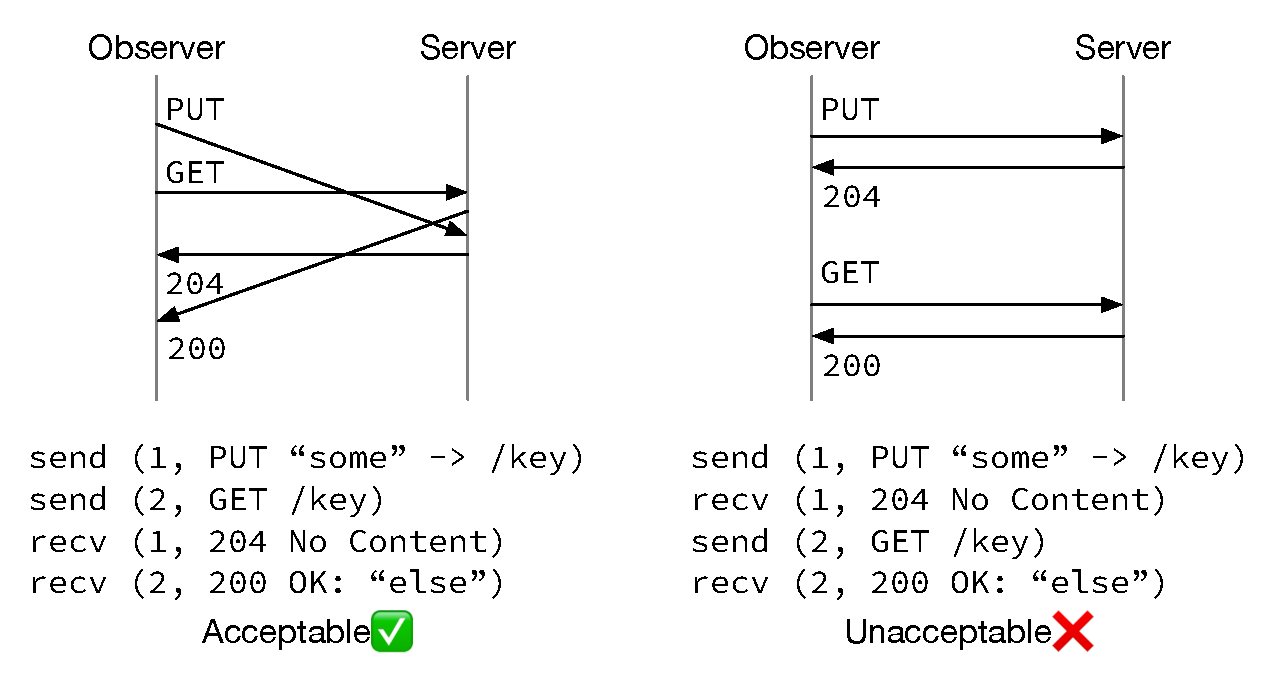
\includegraphics[width=\linewidth]{figures/http-put-bug}
  \caption[GET-after-PUT bug pattern in Apache mutants.]{GET-after-PUT bug
    pattern in Apache mutants.  The trace on the left does not convince the
    tester that the server is buggy, because there exists a certain network
    delay that explains why the PUT request was not reflected in the 200
    response.  When the trace is ordered as shown on the right, the tester
    cannot imagine any network reordering that causes such observation, thus
    must reject the server.}
  \label{fig:put-bug}
\end{figure}
  
\begin{itemize}
  \item Mutants 19 and 20 are related to the WebDAV module, which handles PUT
    requests that modify the target's contents.  The buggy servers wrote to a
    different target from that requested but responds a successful status to
    the client.

    The tester cannot tell that the server is faulty until it queries the
    target's latest contents and observes an unexpected value.  To reject the
    server with full confidence, these observations must be made in a certain
    order, as shown in \autoref{fig:put-bug}.

  \item Mutant 18 is similar to the bug in vanilla Apache: the server should
    have responded with 304 Not Modified but sent back 200 OK instead.  To
    reveal such a violation, a minimal counterexample consists of 4 messages:
    \begin{enumerate}
    \item GET request,
    \item 200 OK response with some ETag \inlinec{"x"},
    \item GET request conditioned over \inlinec{If-None-Match: "x"}, and
    \item 200 OK response, indicating that the ETag \inlinec{"x"} did not match
      itself.
    \end{enumerate}
    Note that (2) must be observed before (3), otherwise the tester will not
    reject the server, with a similar reason as in \autoref{fig:put-bug}.

  \item Mutant 5 is the one shown in \autoref{fig:mutant-example}.  It causes
    the server to skip the return statement when the response should be 404 Not
    Found.  The counterexample can be as small as one GET request on a
    non-existent target, followed by an unexpected response like 403
    Forbidden.  However, my tester generates request targets within a small
    range, so the requests' targets are likely to be created by the tester's
    previous PUT requests.

    Narrowing the range of test case generation might improve the performance in
    aforementioned Mutants 18--20, but Mutant 5 shows that it could also degrade
    the performance of finding some bugs.

  \item The mutants in the proxy module caused the server to forward wrong
    requests or responses.

    To test servers' forward proxying functionality, the tester consists of
    clients and origin servers, both derived by dualization.  When the origin
    server part of the tester accepts a connection from the proxy, it does not
    know for which client the proxy is forwarding requests.  Therefore, the
    tester needs to check the requests sent by all clients, and make sure none
    of them matches the forwarded proxy request.

    The more client connections the tester has created, the longer it takes the
    tester to check all connections before rejecting a buggy proxy.
\end{itemize}

These examples show that the time-consuming issue of some mutants are likely
caused by the generators' heuristics.  Cases like Mutant 5 can be optimized by
state-based heuristics in \autoref{sec:heuristic-state}; Proxy-related bugs can
be more easily found by trace-based heuristics in \autoref{sec:heuristic-trace};
For Mutants 18--20, the requests should be sent at specific time periods so that
the resulting trace is unacceptable per specification, possibly by integrating
packet dynamics~\cite{pkt-dyn} in the test executor.

\section{Testing a File Synchronizer}
\label{sec:sync}

To demonstrate the generality of my specification-based testing methodology, I
also applied it to file synchronizers.  \autoref{sec:file-sut} introduces my
specification of the file system and synchronization semantics.  From these
specifications, I derived a tester program for the Unison file
synchronizer~\cite{unison}, with results shown in \autoref{sec:file-result}.

\subsection{System Under Test}
\label{sec:file-sut}
A file synchronizer manipulates the file system to reconcile updates in
different replicas~\cite{what-sync}.  To check a synchronizer's correctness, the
tester needs to update replicas, launch the synchronization process, and observe
the propagated updates.

\begin{figure}
\begin{coq}
  Inductive node :=
    File      : content          -> node
  | Directory : list (name*node) -> node.

  Context read : path -> node    -> option content.
  Context write: path -> content -> node -> option node.
  Context mkdir: path -> node    -> option node.
  Context ls   : path -> node    -> list name.
  Context rm   : path -> node    -> option node.
\end{coq}
\caption{File system specification.}
\label{fig:file-spec}
\end{figure}

My specification consists of two parts:
\begin{enumerate}
  \item A file system model represented as a tree, where the leaves are files,
    and the branches are directories.  As shown in \autoref{fig:file-spec}, the
    file system model is a simplified abstraction from the POSIX file interface,
    ignoring metadata and file permissions.  Specifying more aspects of the file
    system is discussed in \autoref{chap:discussion}.

    Based on the file system model, I specified five basic file operations that
    the tester may perform: (i) reading contents from a file, (ii) writing
    contents to a file, (iii) creating a new directory, (iv) listing entries
    under a directory, and (v) removing a file or directory recursively.

    Some file operations may fail, \eg, when reading from a path that
    refers to a directory.  These failures are represented as return value
    \ilc{(None: option _)} in the node functions.
  \item A file synchronizer model that syncs updates between two replicas,
    implementing the reconcilation algorithm by \citet{what-sync}:
\begin{coq}
  Definition sigma := node*node*node.
      
  Context reconcile: sigma -> sigma.
\end{coq}
Note that the \ilc{reconcile} function manipulates three replicas.  This is
because the synchronizations might be partial: Upon write-write and write-delete
conflicts, the synchronizer does not propagate the conflicting updates, and
leaves the dirty files untouched in both replicas.

The third parameter of the reconcile function represents the subset of the two
replicas that were synchronized: \ilc{(reconcile (a,b,g))} syncs replicas \ilc a
and \ilc b based on their previous consensus \ilc g.  The consensus is initially
empty and updated when a change in one replica is propagated to another, or the
two replicas have made identical changes.
\end{enumerate}

\begin{figure}
\begin{coq}
  Variant F :=        (* file operations *)
  Fls    (p: path)
| Fread  (p: path)
| Fwrite (p: path) (c: content)
| Fmkdir (p: path)
| Frm    (p: path).

Variant R := R1 | R2. (* replicas      *)

Variant Q :=          (* query type    *)
  QFile (r: R) (f: F)
| QSync.

Variant A :=          (* response type *)
  Als   (l: list name)
| Aread (c: content)
| Aexit (z: Z).       (* exit code     *)
\end{coq}
\caption{Query and response types for testing file synchronizer.}
\label{fig:file-type}
\end{figure}

Having specified the file system interface and the reconciliation semantics, I
modelled the SUT as a deterministic QA server described in
\autoref{def:qaserver}.  As shown in \autoref{fig:file-type}, the request type
\ilc Q can be file operations or the synchronization command; the response type
\ilc A carries the return value of file system queries, or the transactions'
exit code.  For example, when synchronizing the two replicas, code 1 indicates
partial synchronization with conflicts unresolved, and code 2 means the
synchronizer has crashed due to uncaught exceptions or interruptions.

The QA model for the file system+synchronizer was dualized into a tester program
that makes system calls to manipulate files, launch the synchronizer, and
observe the updates.  The system calls are made one at a time, and the file
synchronizer is run as a foreground process that blocks other interactions.
Testing the synchronizer as a nonblocking background process is discussed in
\autoref{chap:discussion}.

\subsection{Experiment Results}
\label{sec:file-result}
The tester rejected the Unison file synchronizer in two ways, and I reported
the counterexample to the developers.  By analyzing the program's behavior, we
determined that one rejection was a valid but defective feature, and the other
rejection was a documented feature not included in my specification.  The
revealed features are as follows:

\paragraph{Synchronizing read-only directories}
When the tester creates a directory in one replica with read and execution
permission (mode \ilj{500}) and calls the synchronization command, Unison
crashed without creating the corresponding directory in the other replica.

The crashing behavior only occurs on macOS, and is caused by Unison's mechanism
for propagating changes: When copying directory \ilj{foo} from replica \ilj A to
replica \ilj B, the synchronizer first creates a temporary directory
``\ilj{B/.unison.foo.xxxx.unison.tmp}'', and then renames it to ``\ilj{B/foo}''.
The \inlinec{rename} implementation in macOS requires write permission to
proceed, so the change was not propagated.

This issue is not considered a violation in Unison or macOS, because: (1) Unison
is allowed to halt without propagating an expected change, as long as its exit
code has indicated an error, and no unexpected change was propagated.  (2) The
POSIX specification~\cite{posix} says the \inlinec{rename} function {\it may}
require write access to the directory.

Despite being compliant to the specification, this feature in Unison is
considered a defect, as it disables synchronization of read-only files and
directories.  A potential fix might be substituting \inlinec{rename} with other
system calls.

This defect was revealed by accident: My file system specification in
\autoref{fig:file-spec} does not mention file permissions, so I defaulted to
mode \ilj{755}.  However, when implementing the test executor, I made a typo
that wrote the permission as hexadecimal \ilc{0x755} while it should be octal
\ilc{0o755}.  This caused the created directory to have mode bits \ilj{525},
which triggered the aforementioned behavior.

This experiment shows that my current abstraction of the file system is worth
expanding to include more information like file permissions, which might reveal
other features of the file synchronizer.

The experiment also reveals a challenge in specifying programs, that the
underlying operating system might also pose uncertainty to the program's
behavior.  Such external nondeterminism may be handled by parameterizing the
program's specification over the OS's, in a similar way as composing the server
model with the network model in \autoref{sec:external-nondet}.

\paragraph{Detecting write-delete conflict}
Suppose replicas \ilj A and \ilj B have a synchronized file \ilj{foo.txt}.  If
the tester deletes \ilj{A/foo.txt} and writes to \ilj{B/foo.txt}, then there is
a conflict between the two replicas.  My specification required Unison to
indicate this conflict with exit code 1.  During the tests, Unison did not
notice that \ilj{B/foo.txt} was changed, decided to propagate the deletion from
replica \ilj A to replica \ilj B, and halted with exit code 2, representing
``non-fatal failures occured during file transfer''.

This behavior is caused by Unison's ``fastcheck'' feature that improves the
performance at the risk of ignoring conflicts.  With fastcheck enabled by
default on *nix systems, the synchronizer detects file modifications by checking
if their timestamps have changed.  When the tester writes to the file within a
short interval, the timestamps might remain unchanged, so the synchronizer
treats the written file as unmodified.  Such behavior can be avoided by updating
the file contents after a longer interval or turning of the preference.

Note that although Unison decided to propagate the file deletion, it does
check the file contents before deleting it.  As a result, the Unison process
crashed and complained that \ilj{B/foo.txt} was modified during synchronization.

If the fastcheck feature was disabled, then Unison can detect the conflict by
comparing the file contents bit-by-bit.  It will propagate no updates and leave
the two replicas as-is, which results the same as enabling fastcheck but at
lower performance.

To include the space of behaviors with fastcheck enabled or upon failing file
transfers, I modified the synchronization semantics in two ways: (1) Instead of
computing the set of all dirty paths and synchronizing all of them, allow
choosing any subset of the dirty paths to synchronize.  (2) If there is a
conflict in the chosen paths, allow halting the synchronizer with exit code 1
(conflict detected) or 2 (propagation failed).  The loosened specification
accepted all behavior it observed from Unison.

These experiments show that my testing methodology can effectively reject
implementations that do not comply with the specification.  The incompliance
indicates that either (i) the implementation does not conform with the protocol,
\eg, Apache and Nginx violating RFC 7232, or (2) the specification is
incorrect, \eg, my initial file synchronizer specification not modeling all
features of Unison.  Automatically detecting the incompliances helps developers
to correctly specify and implement systems in real-world practices.
